\chapter{Sezioni Trasversali}

È possibile ottenere le sezioni trasversali del tracciato utilizzando il comando Corridors/Dynamic Section, ed è anche possibile visualizzare sulla sezione anche le aree e i relativi volumi di scavo e riporto.

\begin{figure}[H]
	\centering
	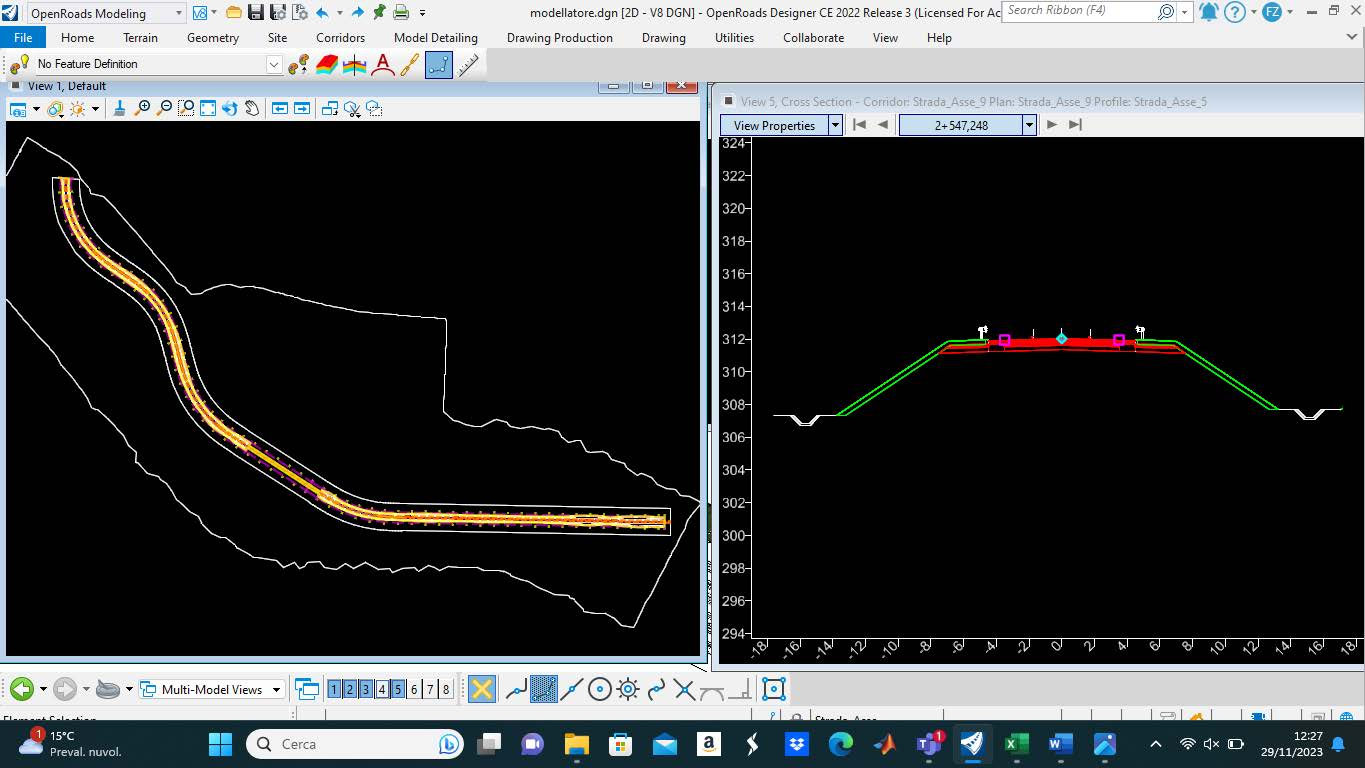
\includegraphics[width=\linewidth]{Figures/Sezione in rilevato}
	\captionof{figure}{Sezione in rilevato}
    \label{fig:Sezione in rilevato}
\end{figure}

\begin{figure}[H]
	\centering
	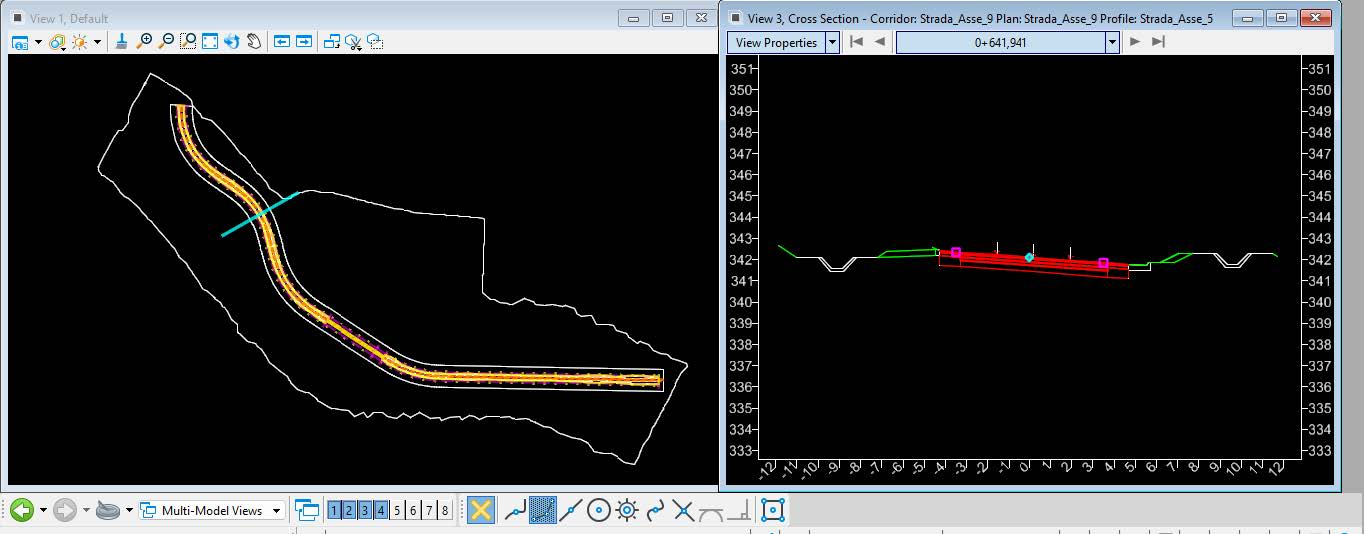
\includegraphics[width=\linewidth]{Figures/Sezione a mezzacosta}
	\captionof{figure}{Sezione a mezzacosta}
    \label{fig:Sezione a mezzacosta}
\end{figure}

\begin{figure}[H]
	\centering
	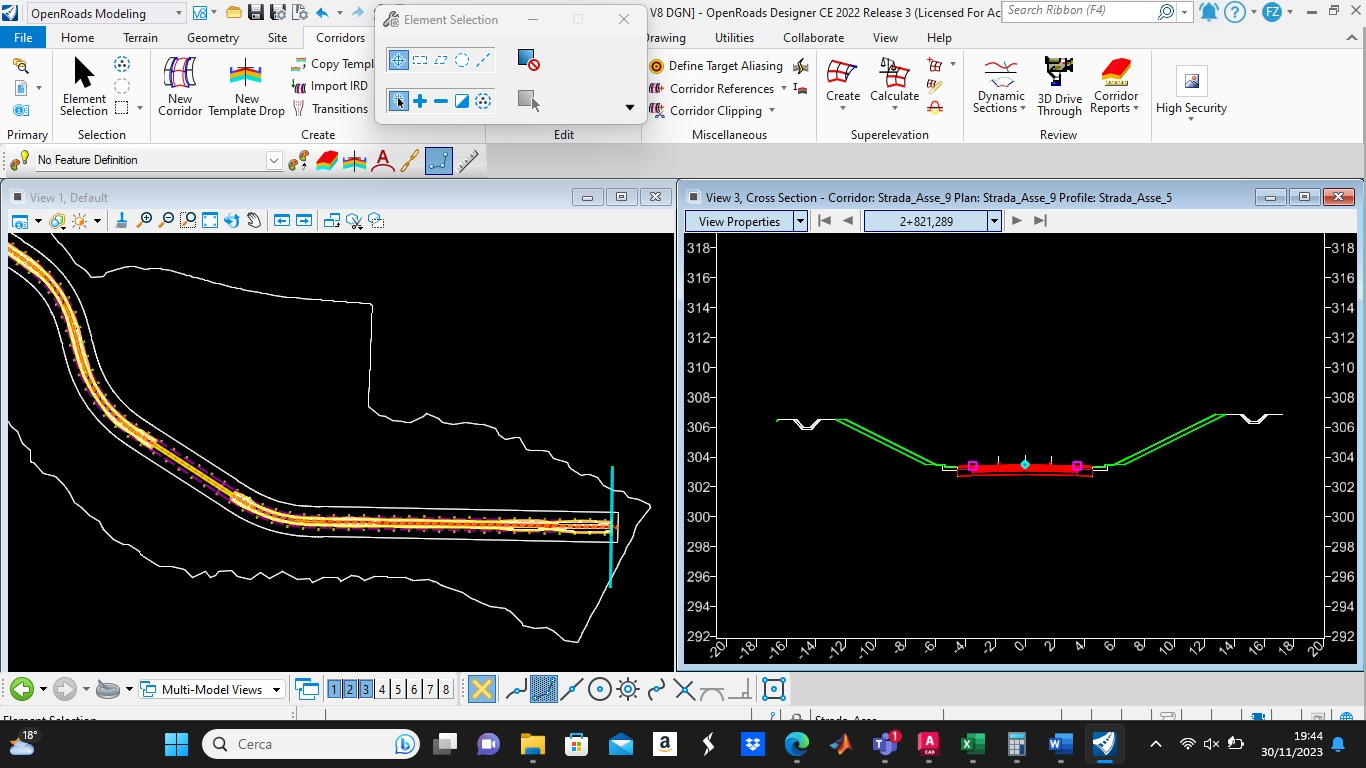
\includegraphics[width=\linewidth]{Figures/Sezione in trincea}
	\captionof{figure}{Sezione in trincea}
    \label{fig:Sezione in trincea}
\end{figure}

Attraverso il report del corridor è possibile, inoltre vedere quanto è il volume di scavo e di riporto complessivo o di ogni singola sezione.

\begin{figure}[H]
	\centering
	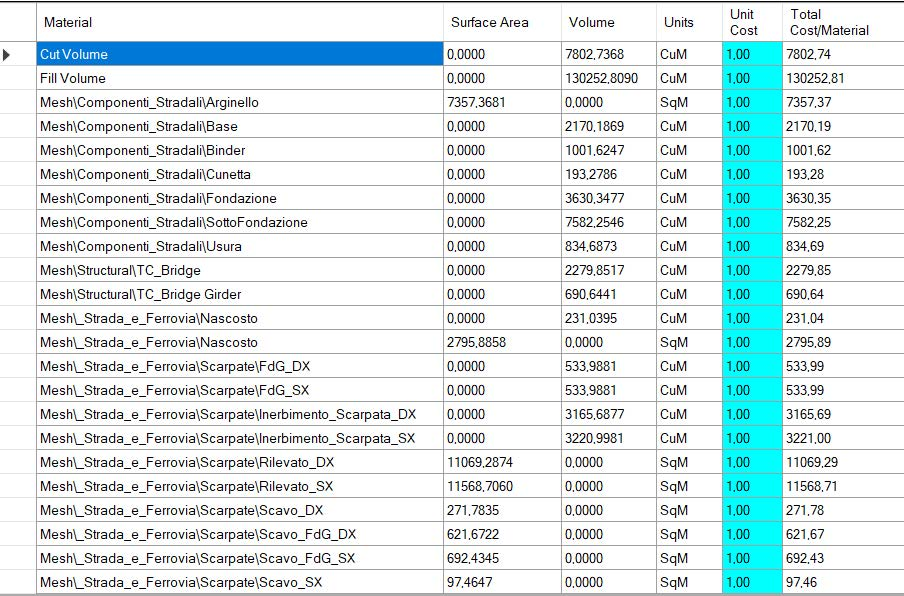
\includegraphics[width=\linewidth]{Figures/Corridor report}
	\captionof{figure}{Corridor report}
    \label{fig:Corridor report}
\end{figure}



